%!TEX root = ../paper.tex
\chapter{程序运行效果}
	\section{星座图}
		\par 在电脑上,如果程序正常运行,则可以在接收端看到如图\ref{fig:dvbt_rx_map_1}和\ref{fig:dvbt_rx_map_2}星座图。
		\begin{figure}[htp]
			\centering
			\subfigure[DVB-T接收端星座图]{%
				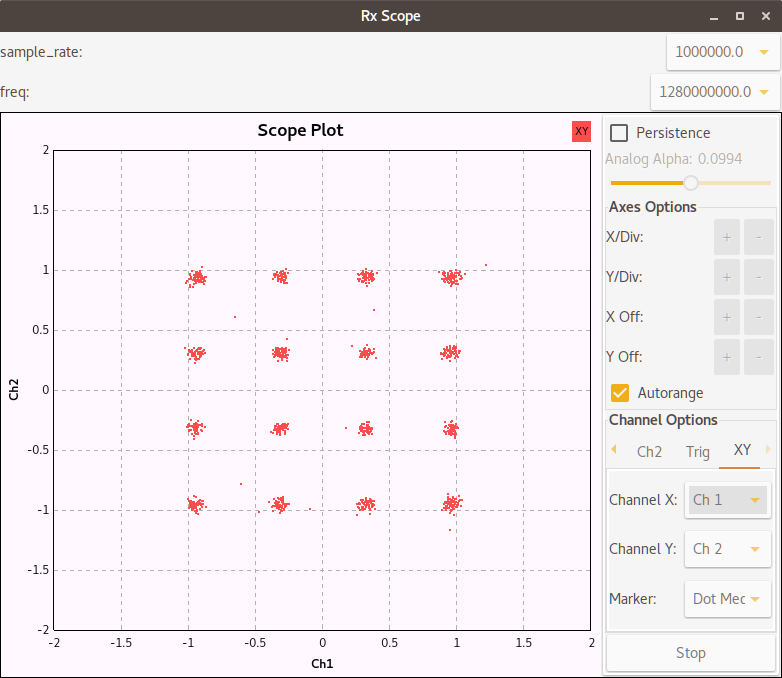
\includegraphics[width=0.4\textwidth]{figures/dvbt_rx_map_1.png}
				\label{fig:dvbt_rx_map_1}}
			\subfigure[DVB-T接收端星座图]{%
				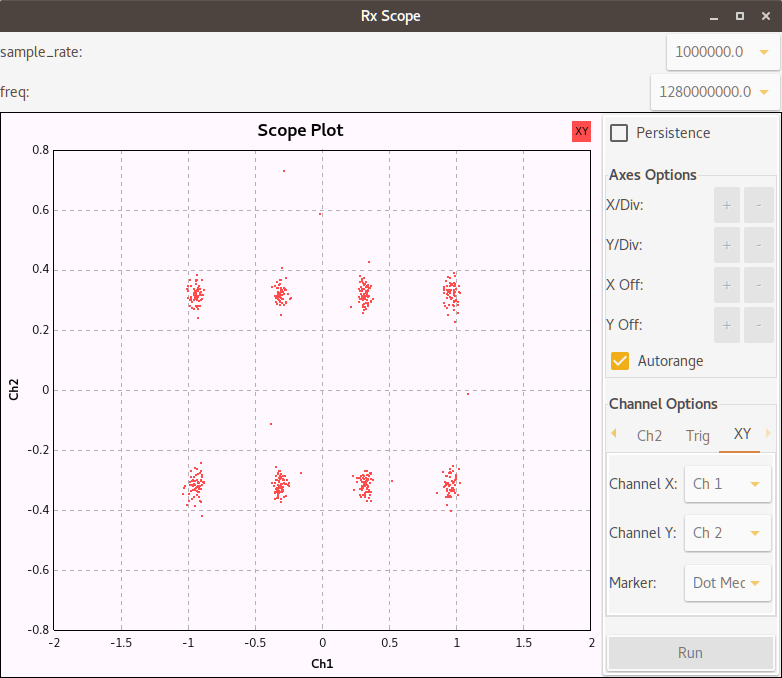
\includegraphics[width=0.4\textwidth]{figures/dvbt_rx_map_2.png}
				\label{fig:dvbt_rx_map_2}} \\
		\end{figure}
	\section{频谱}
		\par 有如下几种方式查看输出频谱:
		\par $\bullet$ 使用GNU Radio构建一个简易的频谱仪。
		\par 按图搭建框图\ref{fig:dvbt_rx_fft}即可,其效果如图\ref{fig:dvbt_rx_fft_1}所示。
		\begin{figure}[htp]
			\centering
			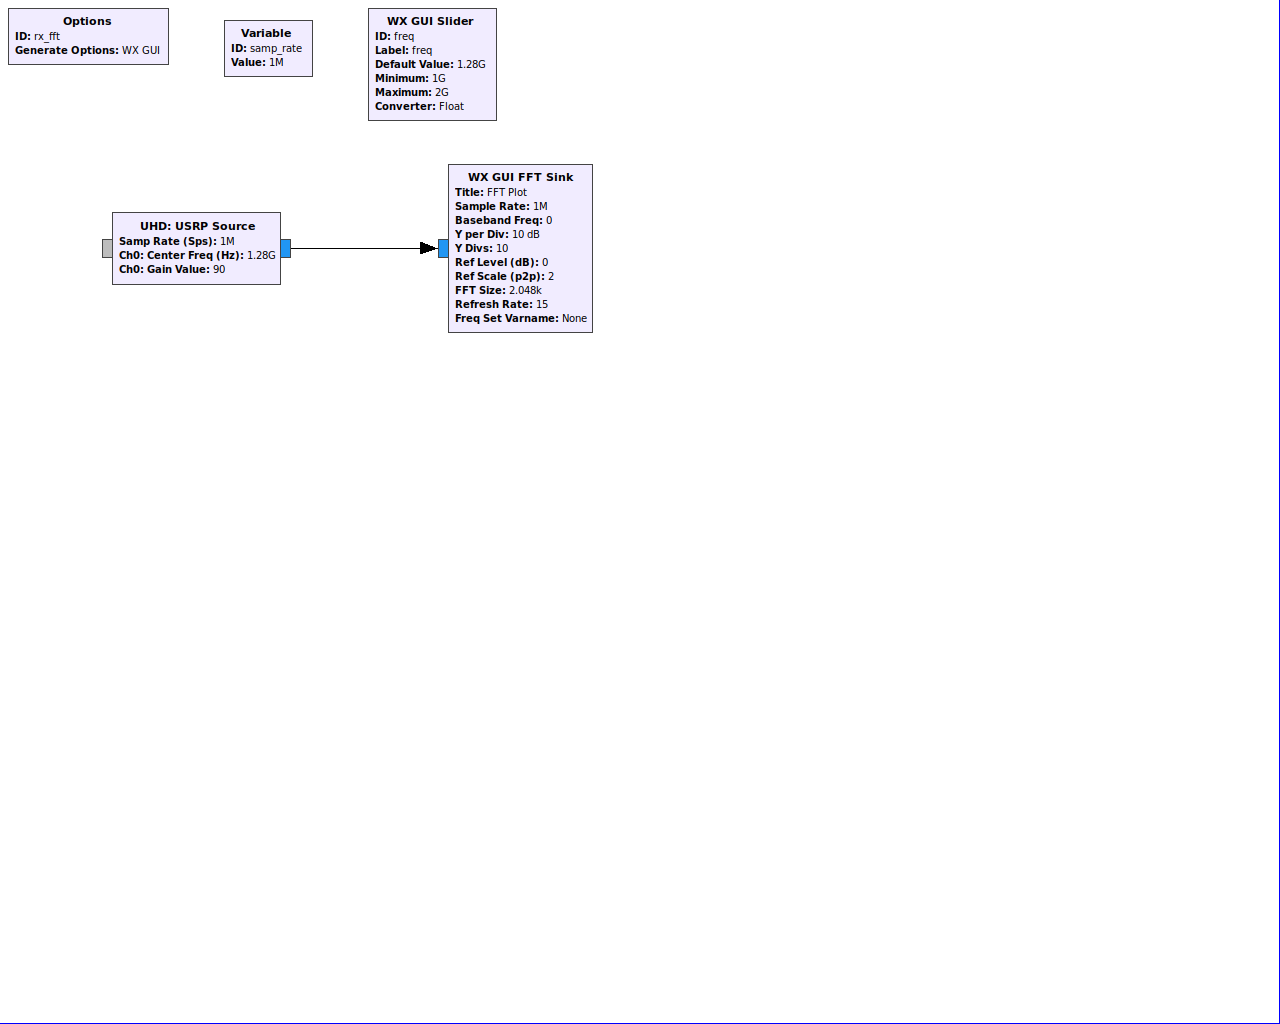
\includegraphics[width=13cm]{figures/dvbt_rx_fft.png}
			\caption{GNU Radio频谱仪}
			\label{fig:dvbt_rx_fft}
		\end{figure}
		\begin{figure}[htp]
			\centering
			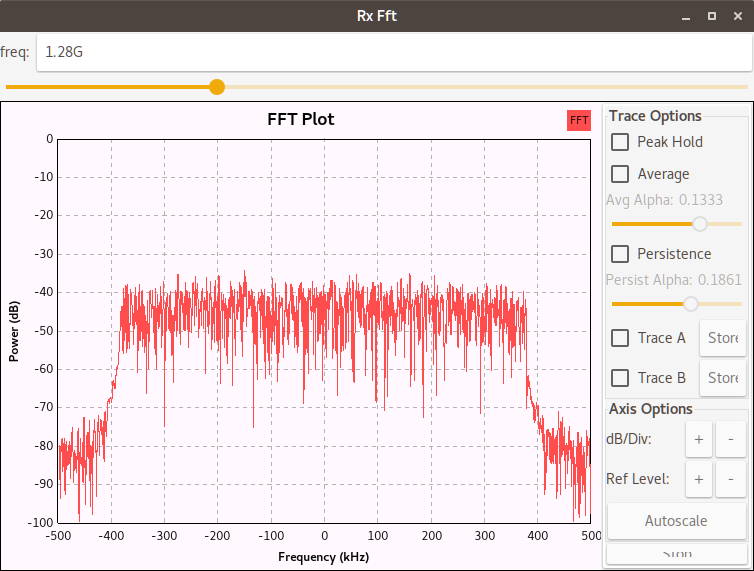
\includegraphics[width=13cm]{figures/dvbt_rx_fft_1.png}
			\caption{GNU Radio频谱仪}
			\label{fig:dvbt_rx_fft_1}
		\end{figure}
		\par $\bullet$ 使用频谱仪
		\par 带宽为2MHz时频谱如图\ref{fig:dvbt_BW_2MHz}所示,带宽为5MHz时频谱如图\ref{fig:dvbt_BW_5MHz}所示。
		\begin{figure}[htp]
			\centering
			\subfigure[带宽为2MHz时频谱]{%
				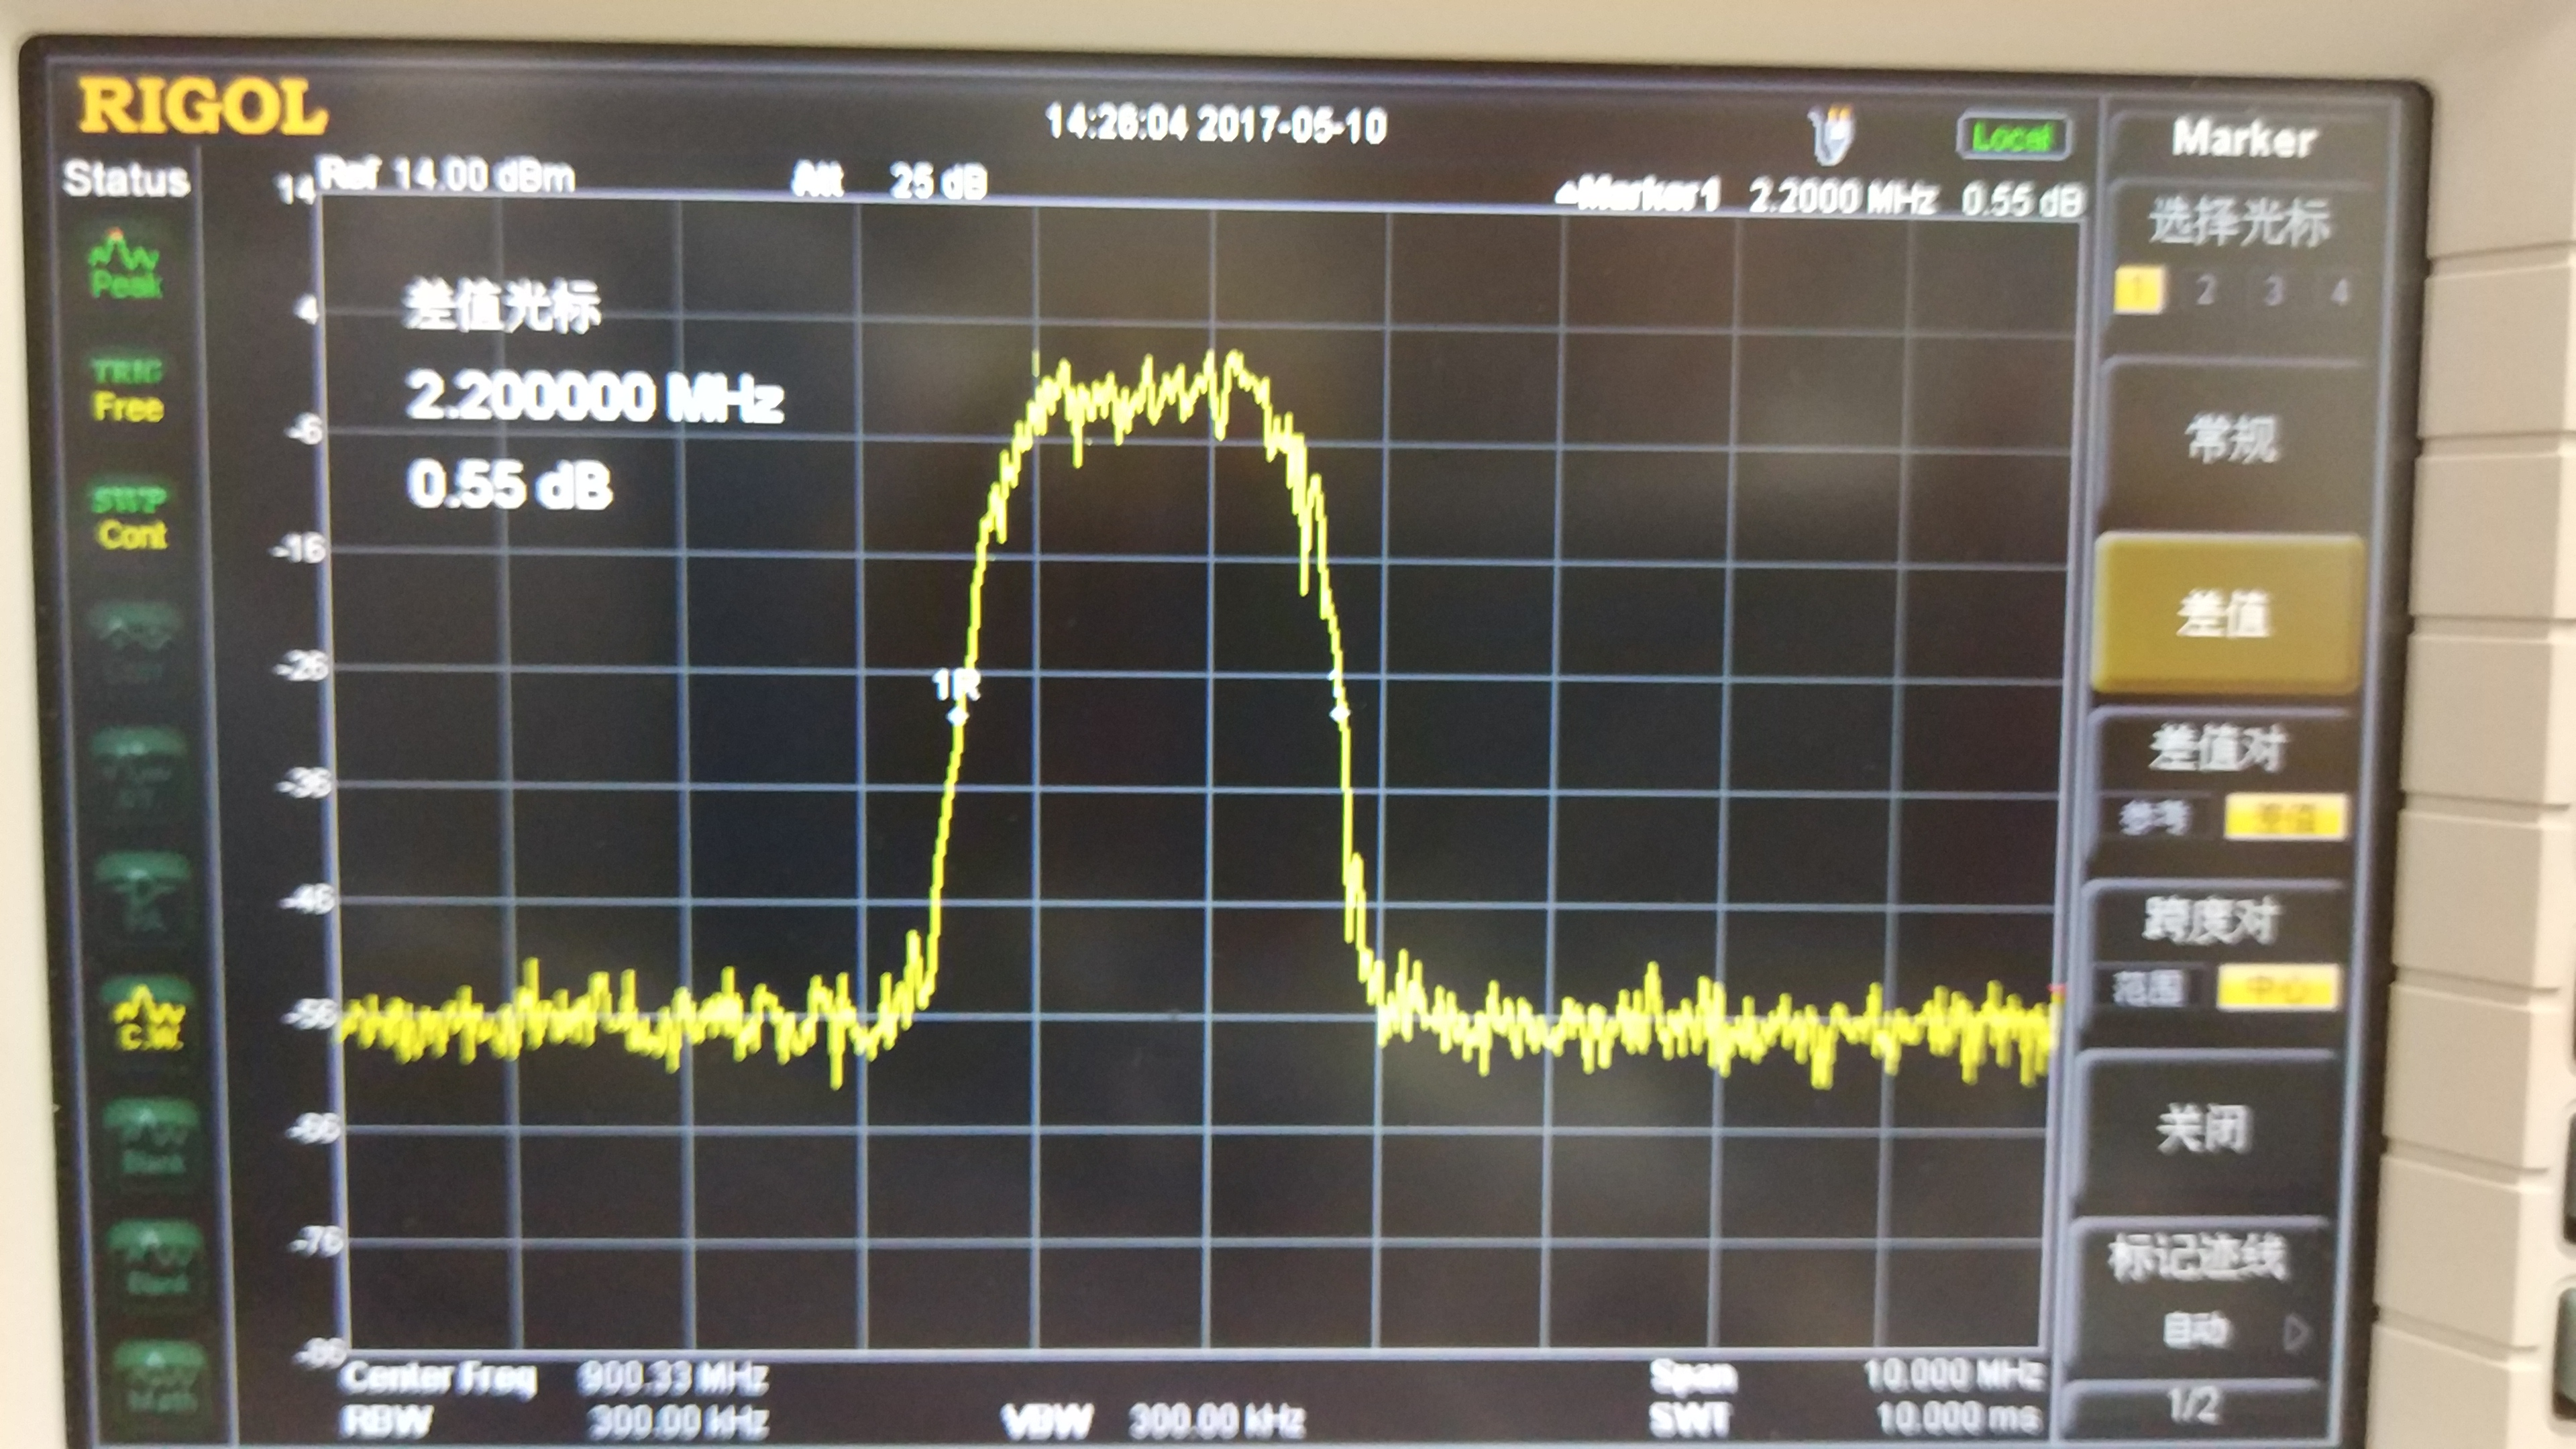
\includegraphics[width=0.4\textwidth]{figures/dvbt_BW_2MHz.jpg}
				\label{fig:dvbt_BW_2MHz}}
			\subfigure[带宽为5MHz时频谱]{%
				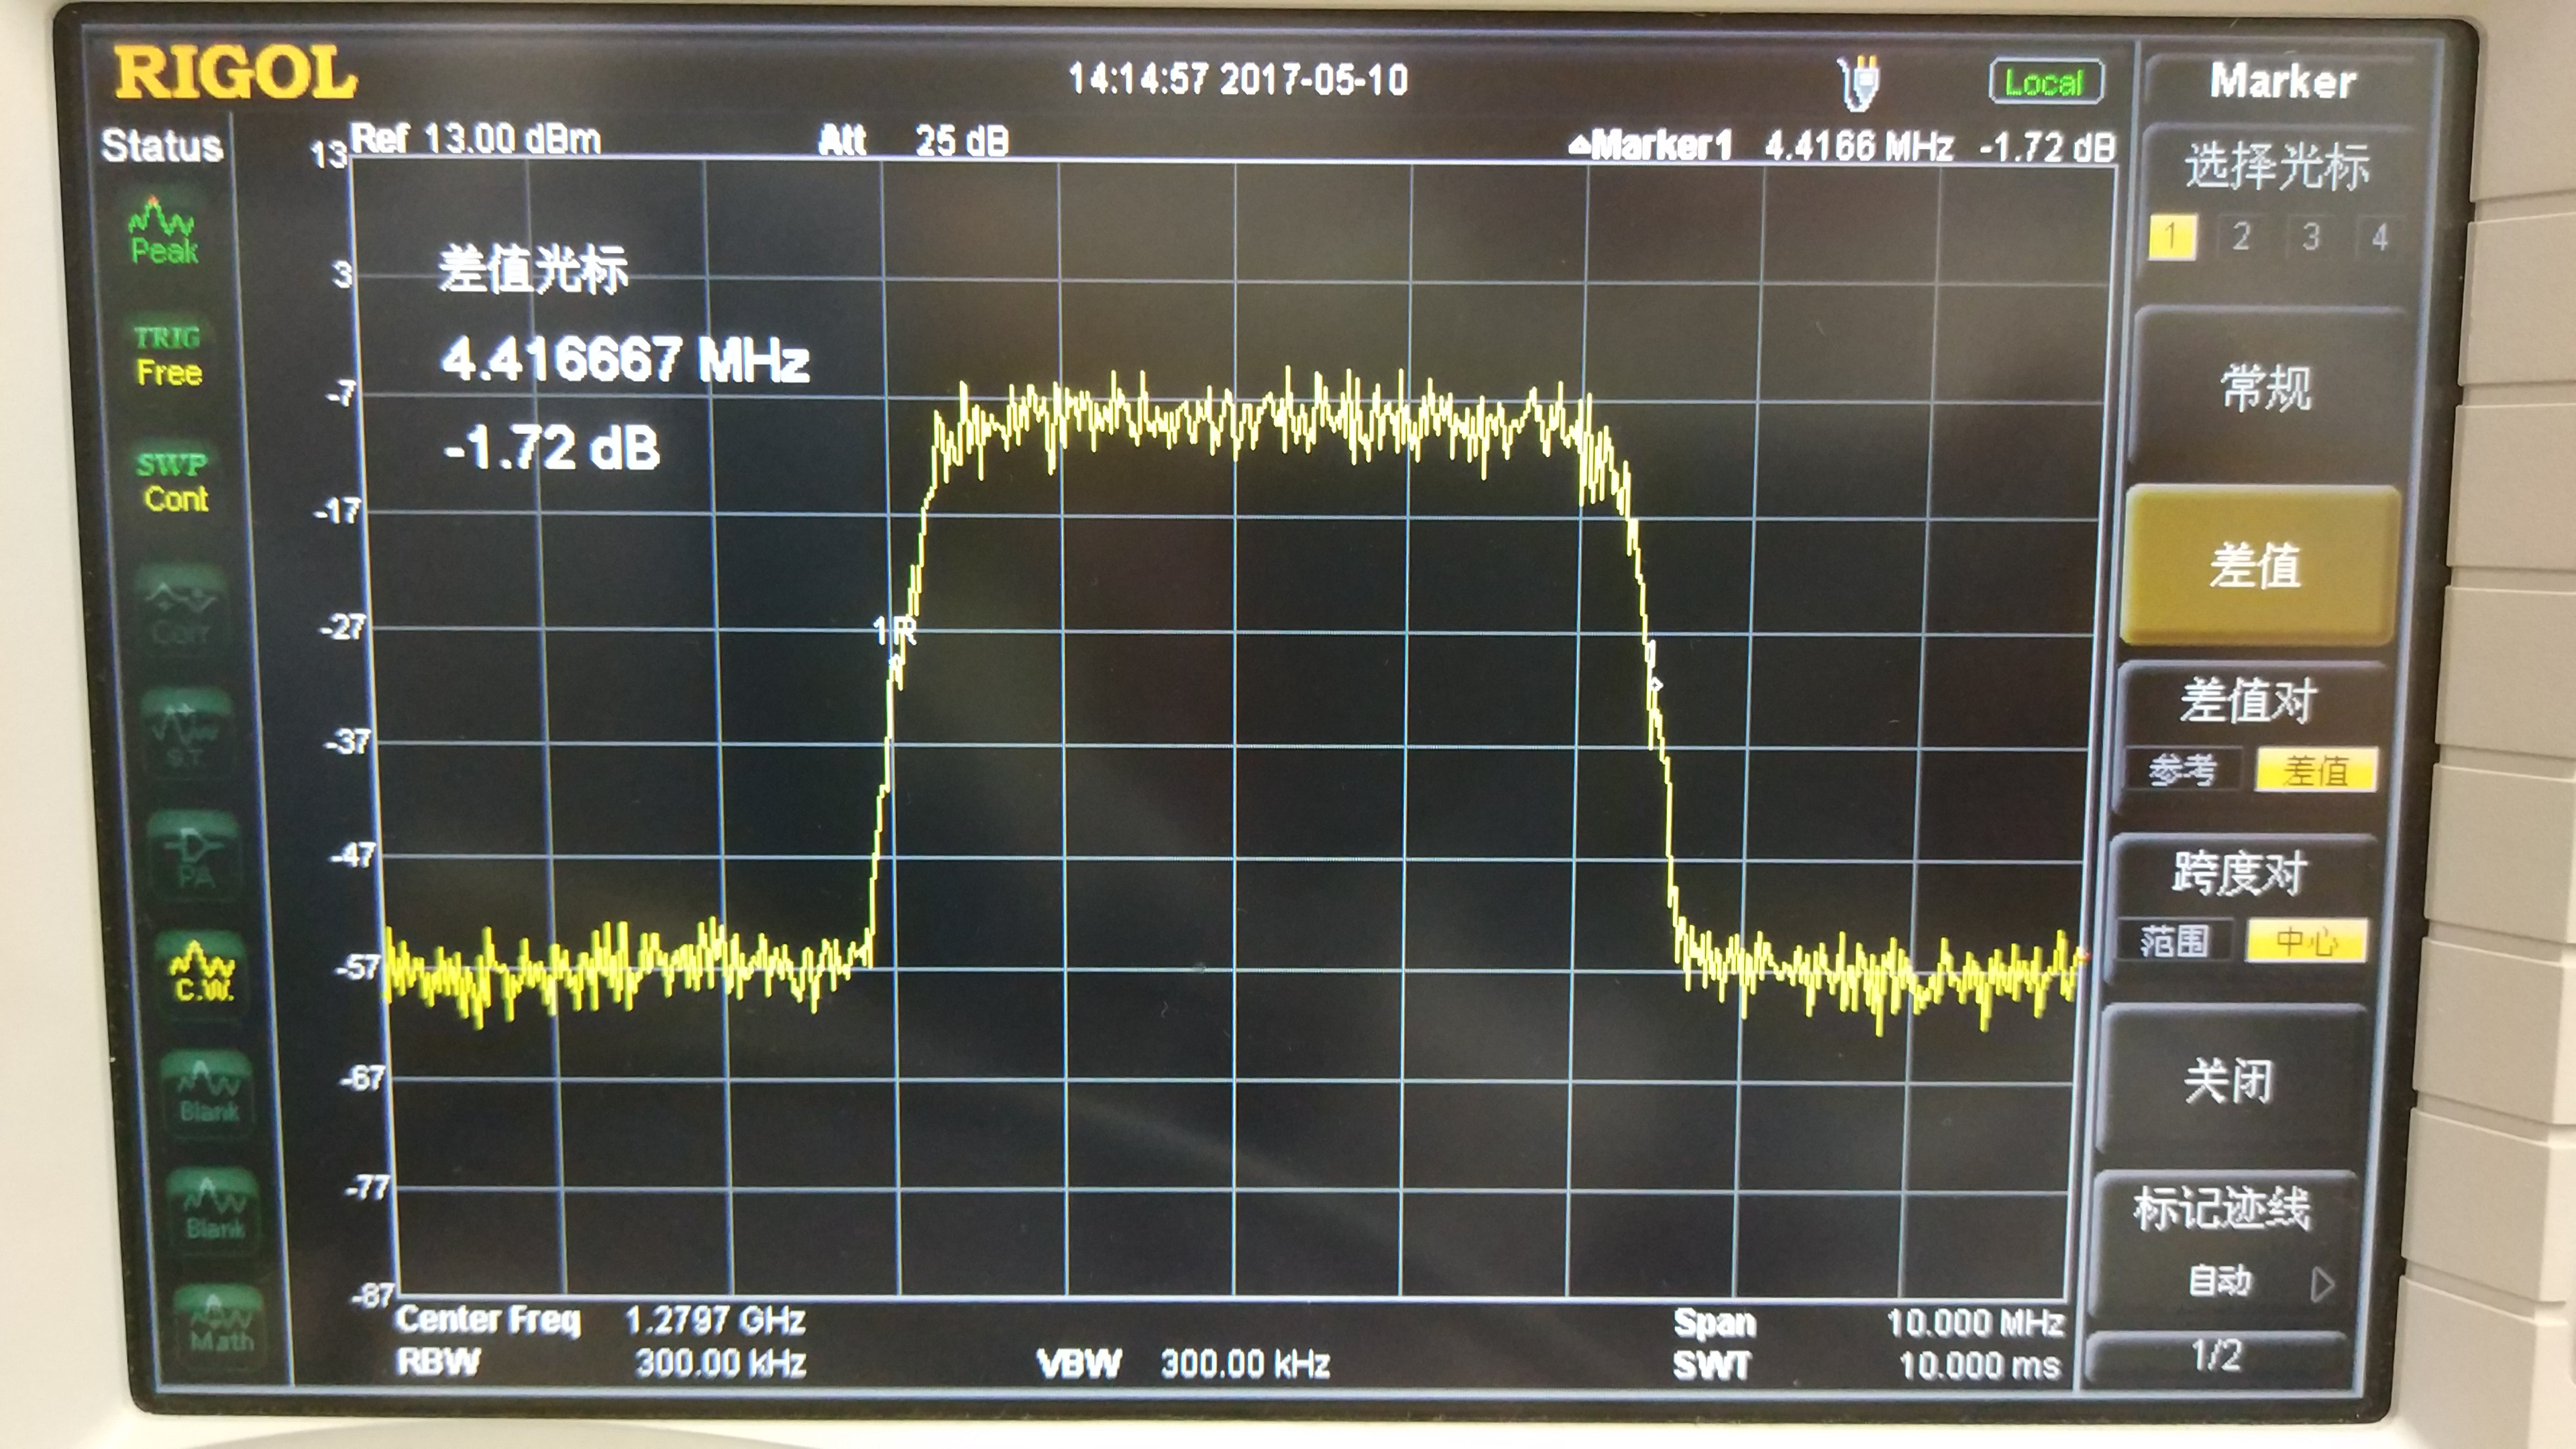
\includegraphics[width=0.4\textwidth]{figures/dvbt_BW_5MHz.jpg}
				\label{fig:dvbt_BW_5MHz}} \\
		\end{figure}
		\par $\bullet$ 使用gqrx
		\par 直接在gqrx中调节到相应频段查看即可,不再赘述。
	\section{距离}
		\par 收发端之间距离较近时可以在当前目录下看到生成的\lstinline[language=sh]{test_out.ts}文件,使用VLC或者Mplayer可以播放出视频,如图\ref{fig:dvbt_rx_TS}。
		\begin{figure}[htp]
			\centering
			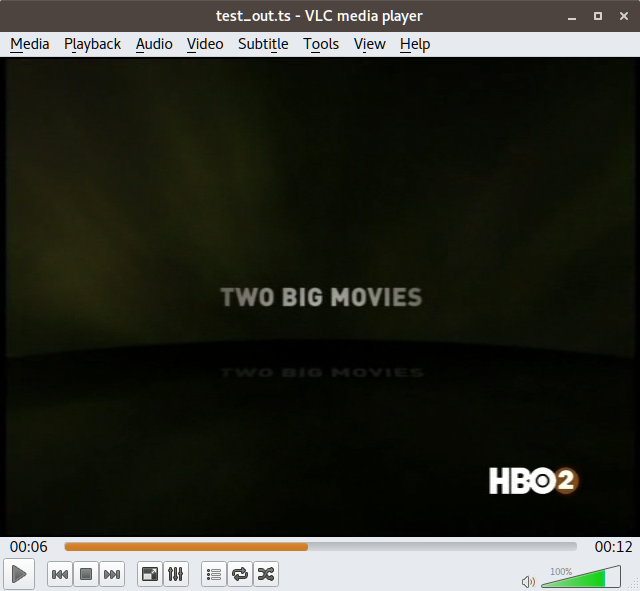
\includegraphics[width=13cm]{figures/dvbt_rx_TS.png}
			\caption{视频输出}
			\label{fig:dvbt_rx_TS}
		\end{figure}
		\par 由于USRP的输出功率,信号能传播大约一间屋子的距离(约5米),超过这段距离将会出现以如图\ref{fig:dvbt_rx_2MHz_ranged_2}无法解星座映射以及如图\ref{fig:dvbt_rx_TS_broken}视频播放失真的情况。
		\begin{figure}[htp]
			\centering
			\subfigure[约5m处星座图]{%
				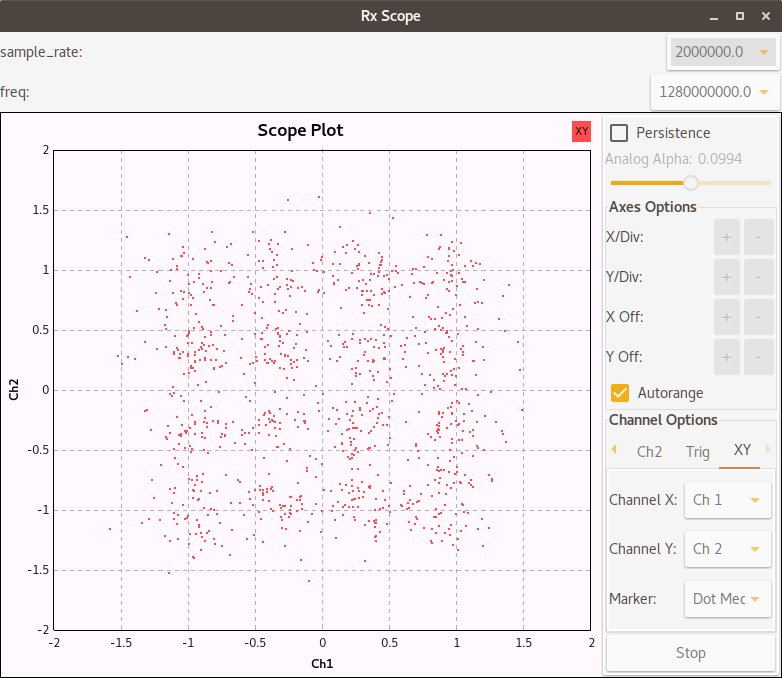
\includegraphics[width=0.4\textwidth]{figures/dvbt_rx_2MHz_ranged_2.png}
				\label{fig:dvbt_rx_2MHz_ranged_2}}
			\subfigure[约5m处视频播放]{%
				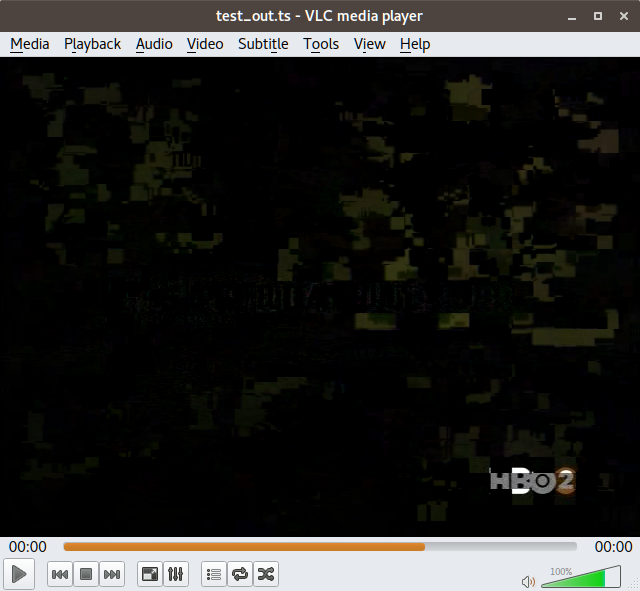
\includegraphics[width=0.4\textwidth]{figures/dvbt_rx_TS_broken.png}
				\label{fig:dvbt_rx_TS_broken}} \\
		\end{figure}
	\section{采样率}
		\label{sec:sample_rate}
		\par 在实验中可以看到影响带宽的因素为UHD\_Sink模块中的采样率,查阅众多资料后才有了一些暂未经证实的推测,提供以下思路,供后续开发者参考。
		\par UHD\_Sink中的采样率可以理解为传送的数据的大小,本设计中为每秒送给USRP的数据量的大小,数据为复数形式,其中实部作为I路,虚部作为Q路送入,所以每一个信号对应一个子载波信息。在5MHz采样率下整个系统要求的输出为每秒5M个复数,即系统每秒要输出约5M*4Byte=20MB(在GNU Radio中gr\_complex等同于std::complex<float>)数据即5MS/s @ 16-bit I/Q(I、Q各16bit,complex实部虚部各占16bit,2Byte)。为了提供这么多的输出,前面的过程将要进行大量的运算,可能已经达到计算机处理的瓶颈,并且USB2.0能传输的最大带宽为8MS/s @ 16-bit I/Q,所以在性能一定时限制整个系统带宽的主要因素就是该采样率。如若需要更高的采样率只能使用更快的CPU或者使用FPGA来进行计算,同时使用USB3.0协议或者通过以太网口进行数据传输。
		\par DVB-T系统要求的带宽要最小为6MHz,而该系统在稳定传输时的带宽仅为5MHz,传输1秒视频的时间大于1秒,也就解释了视频无法实时播放的原因。
		\par 这种视频无法实时播放的情况也从佐证了该系统可以用于传输特定数据信号的观点,为后续开发提供了一定基础。
	\section{树莓派发射}
		\par 将设备按图\ref{fig:dvbt_raspi}所示连接,便可以在接收端上看到\lstinline[language=sh]{test_out.ts}但是由于带宽太小,误码率高,在OFDM接收端处无法解码,该文件无法流畅播放。
		\par 由于树莓派的计算性能与IO性能较弱,仅能提供约500KHz的带宽,如图\ref{fig:dvbt_raspi_bandwidth},也许将部分模块交由FPGA处理会有巨大的提升,或者通过gpu来计算相关模块,或者在要求不高的情况下去除一些编码交织模块,有待后续开发者继续研究。
		\begin{figure}[htp]
			\centering
			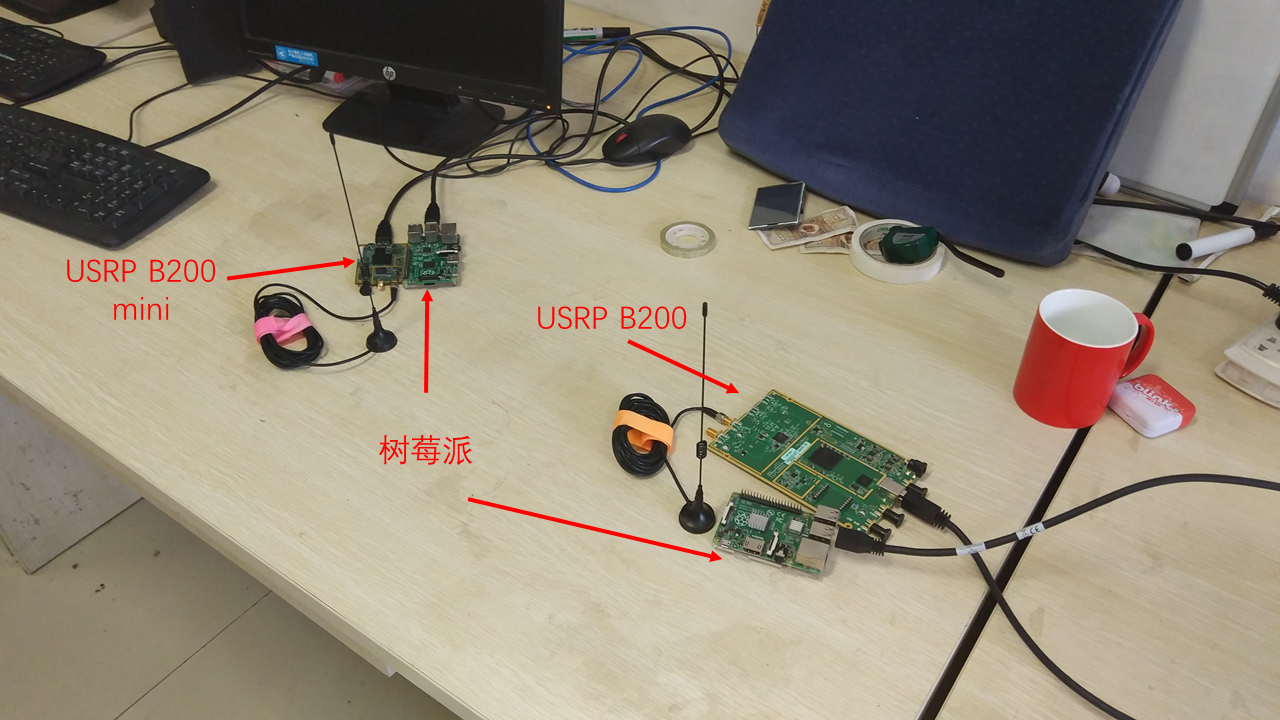
\includegraphics[width=13cm]{figures/dvbt_raspi.png}
			\caption{树莓派连接图}
			\label{fig:dvbt_raspi}
		\end{figure}
		\begin{figure}[htp]
			\centering
			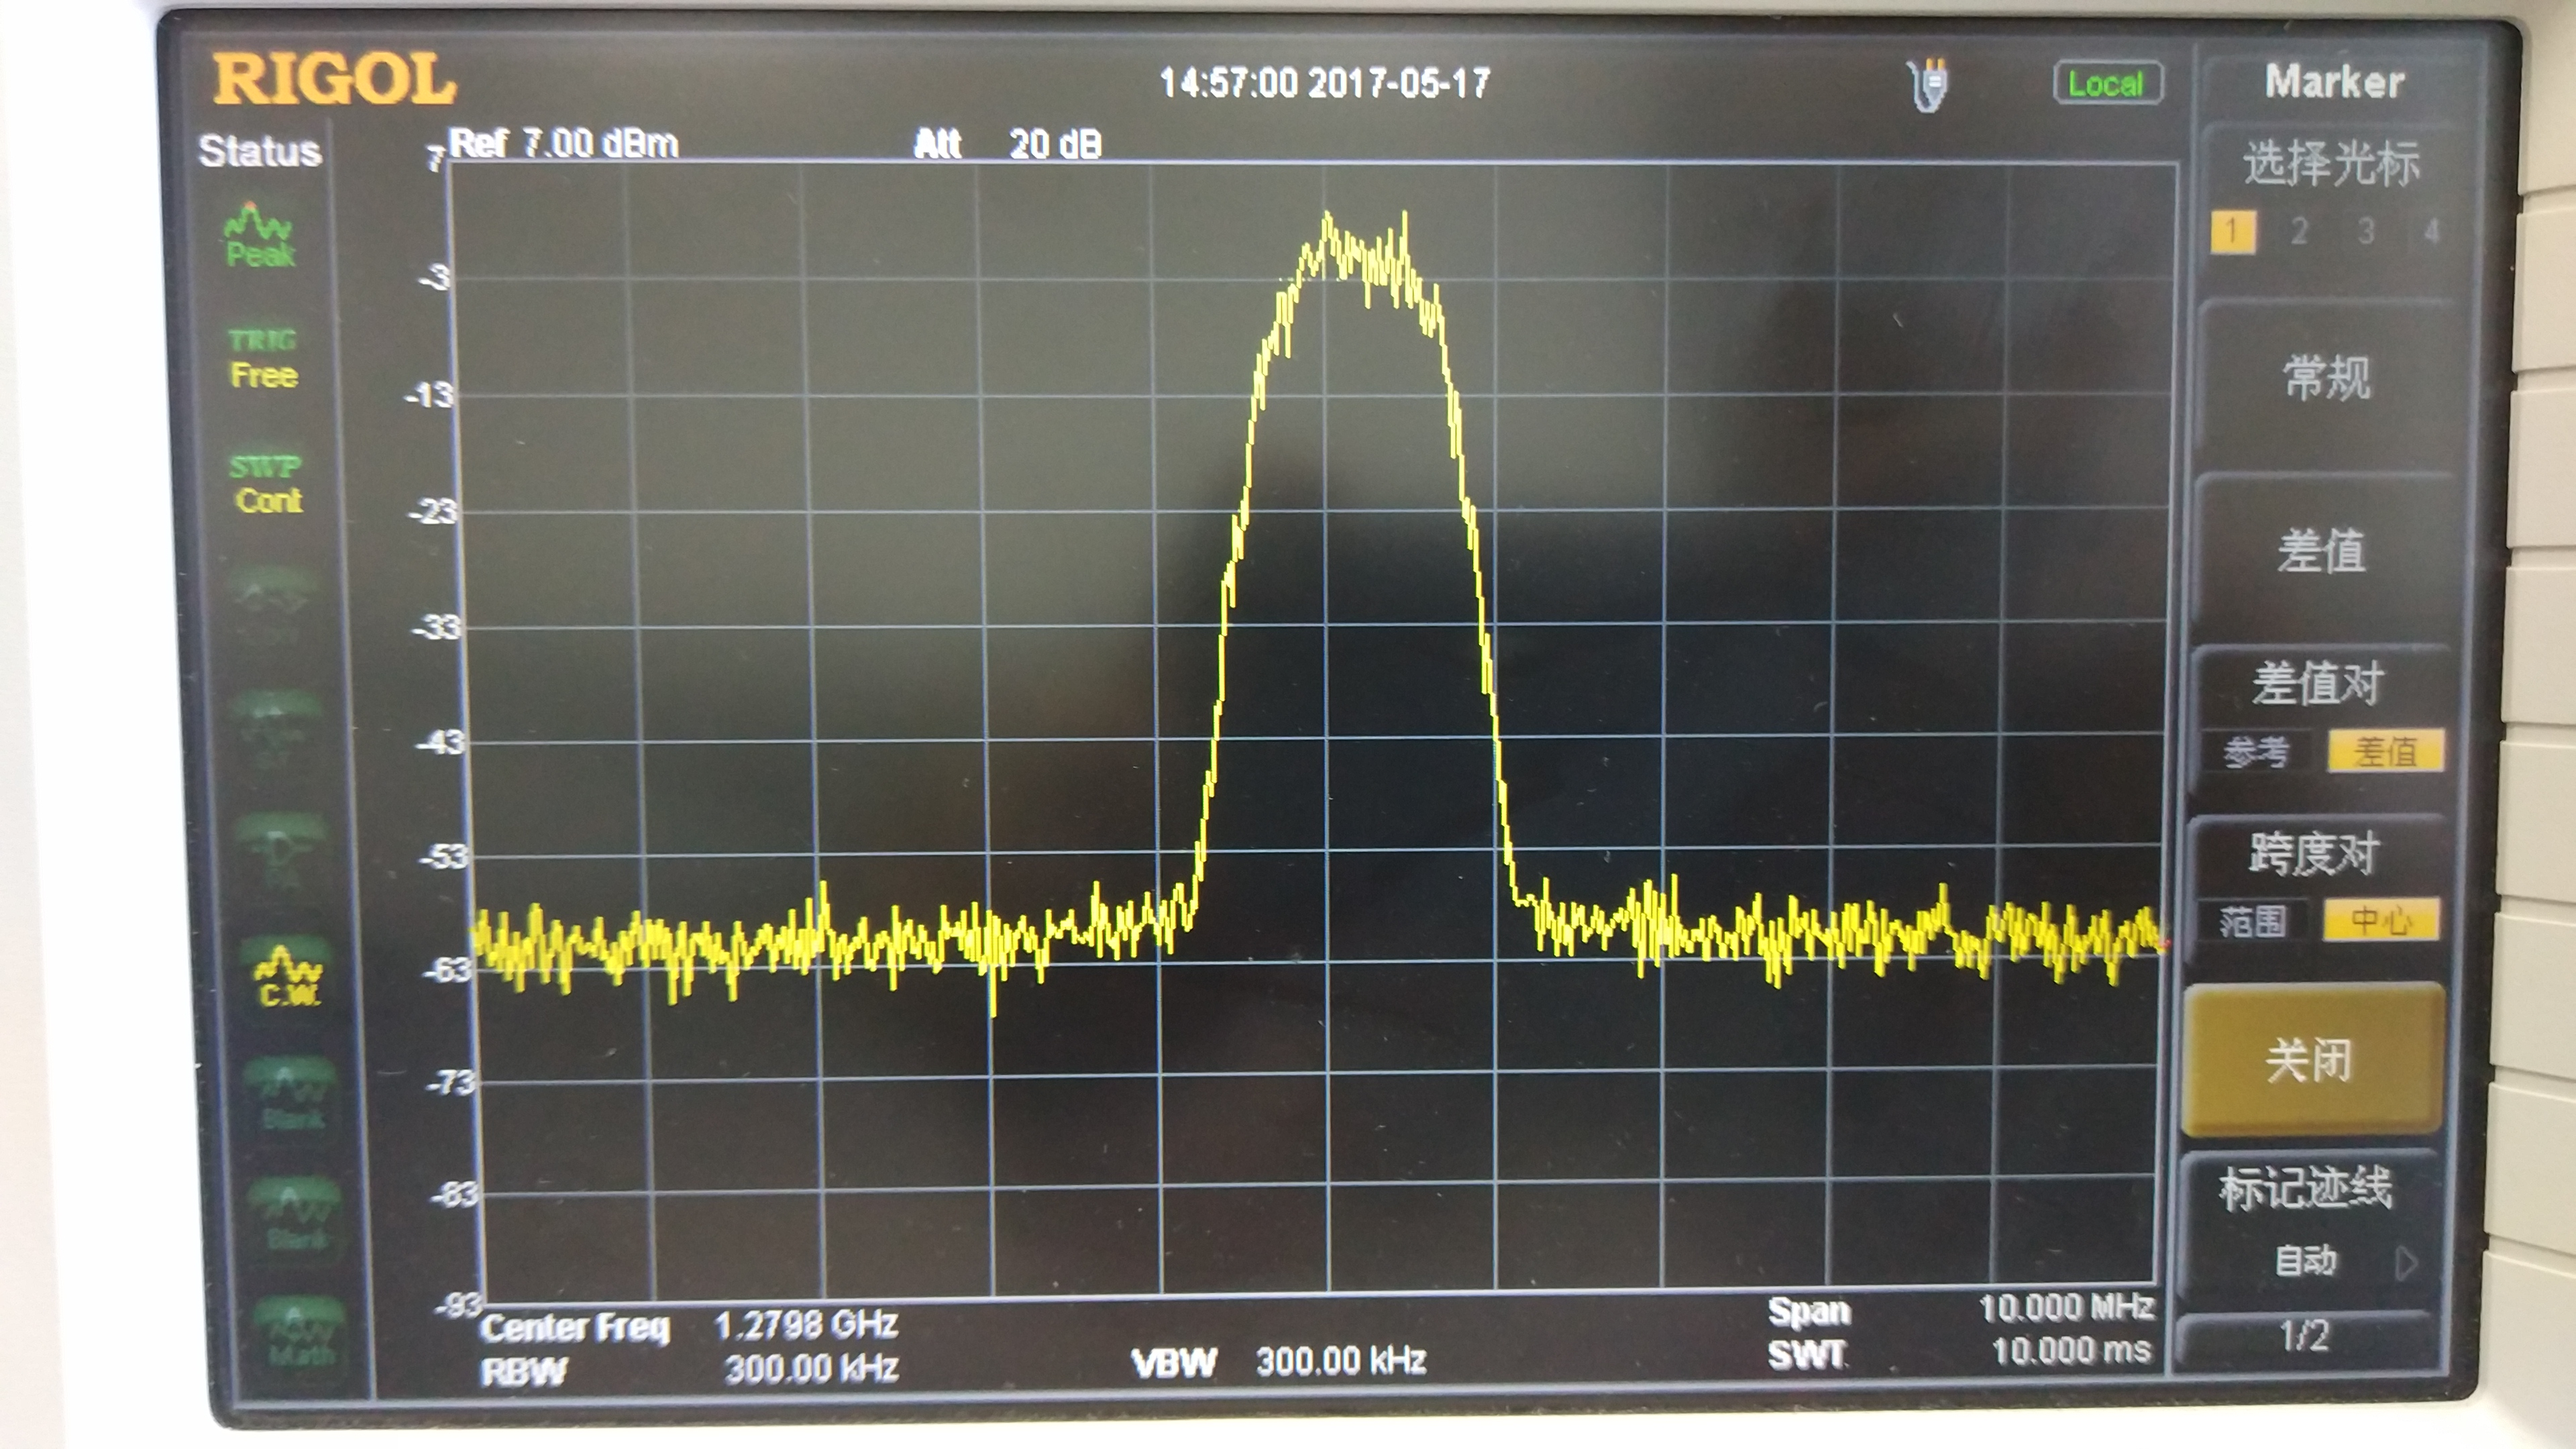
\includegraphics[width=13cm]{figures/dvbt_raspi_bandwidth.jpg}
			\caption{树莓派运行频谱}
			\label{fig:dvbt_raspi_bandwidth}
		\end{figure}
		% \begin{figure}[htp]
		% 	\centering
		% 	\subfigure[树莓派连接图]{%
		% 		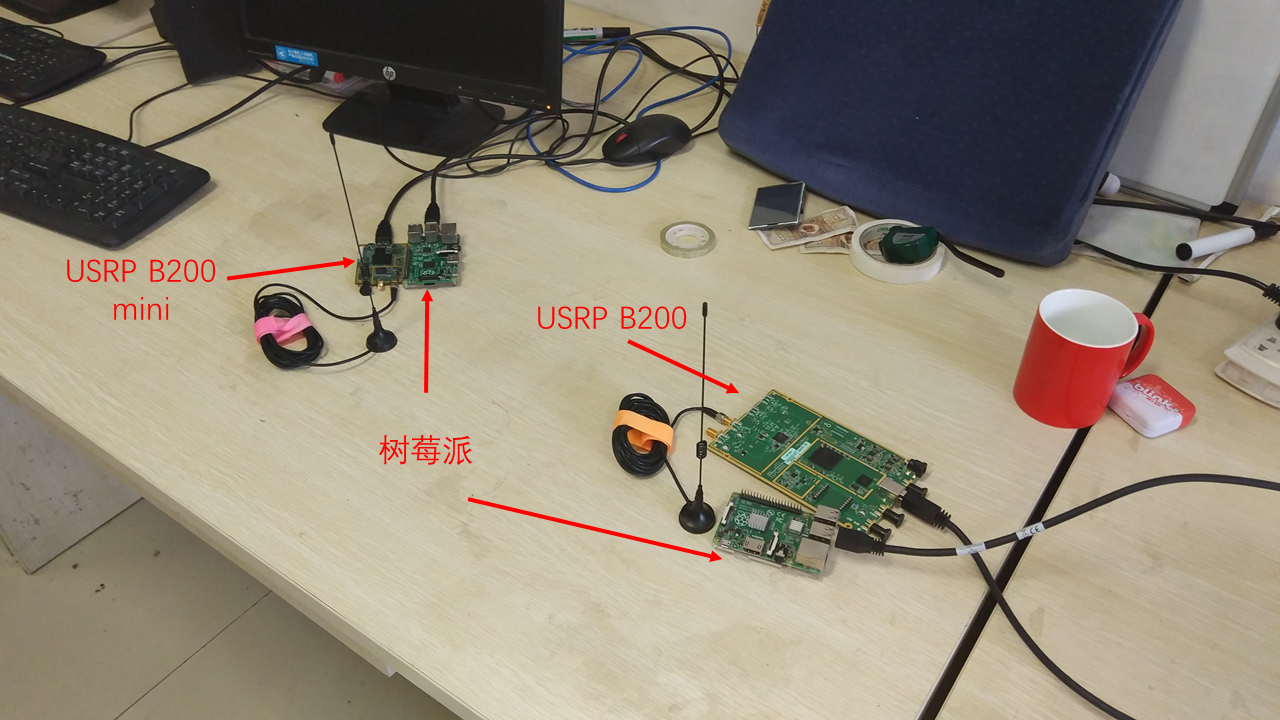
\includegraphics[width=0.4\textwidth]{figures/dvbt_raspi.png}
		% 		\label{fig:dvbt_raspi}}
		% 	\subfigure[树莓派运行频谱]{%
		% 		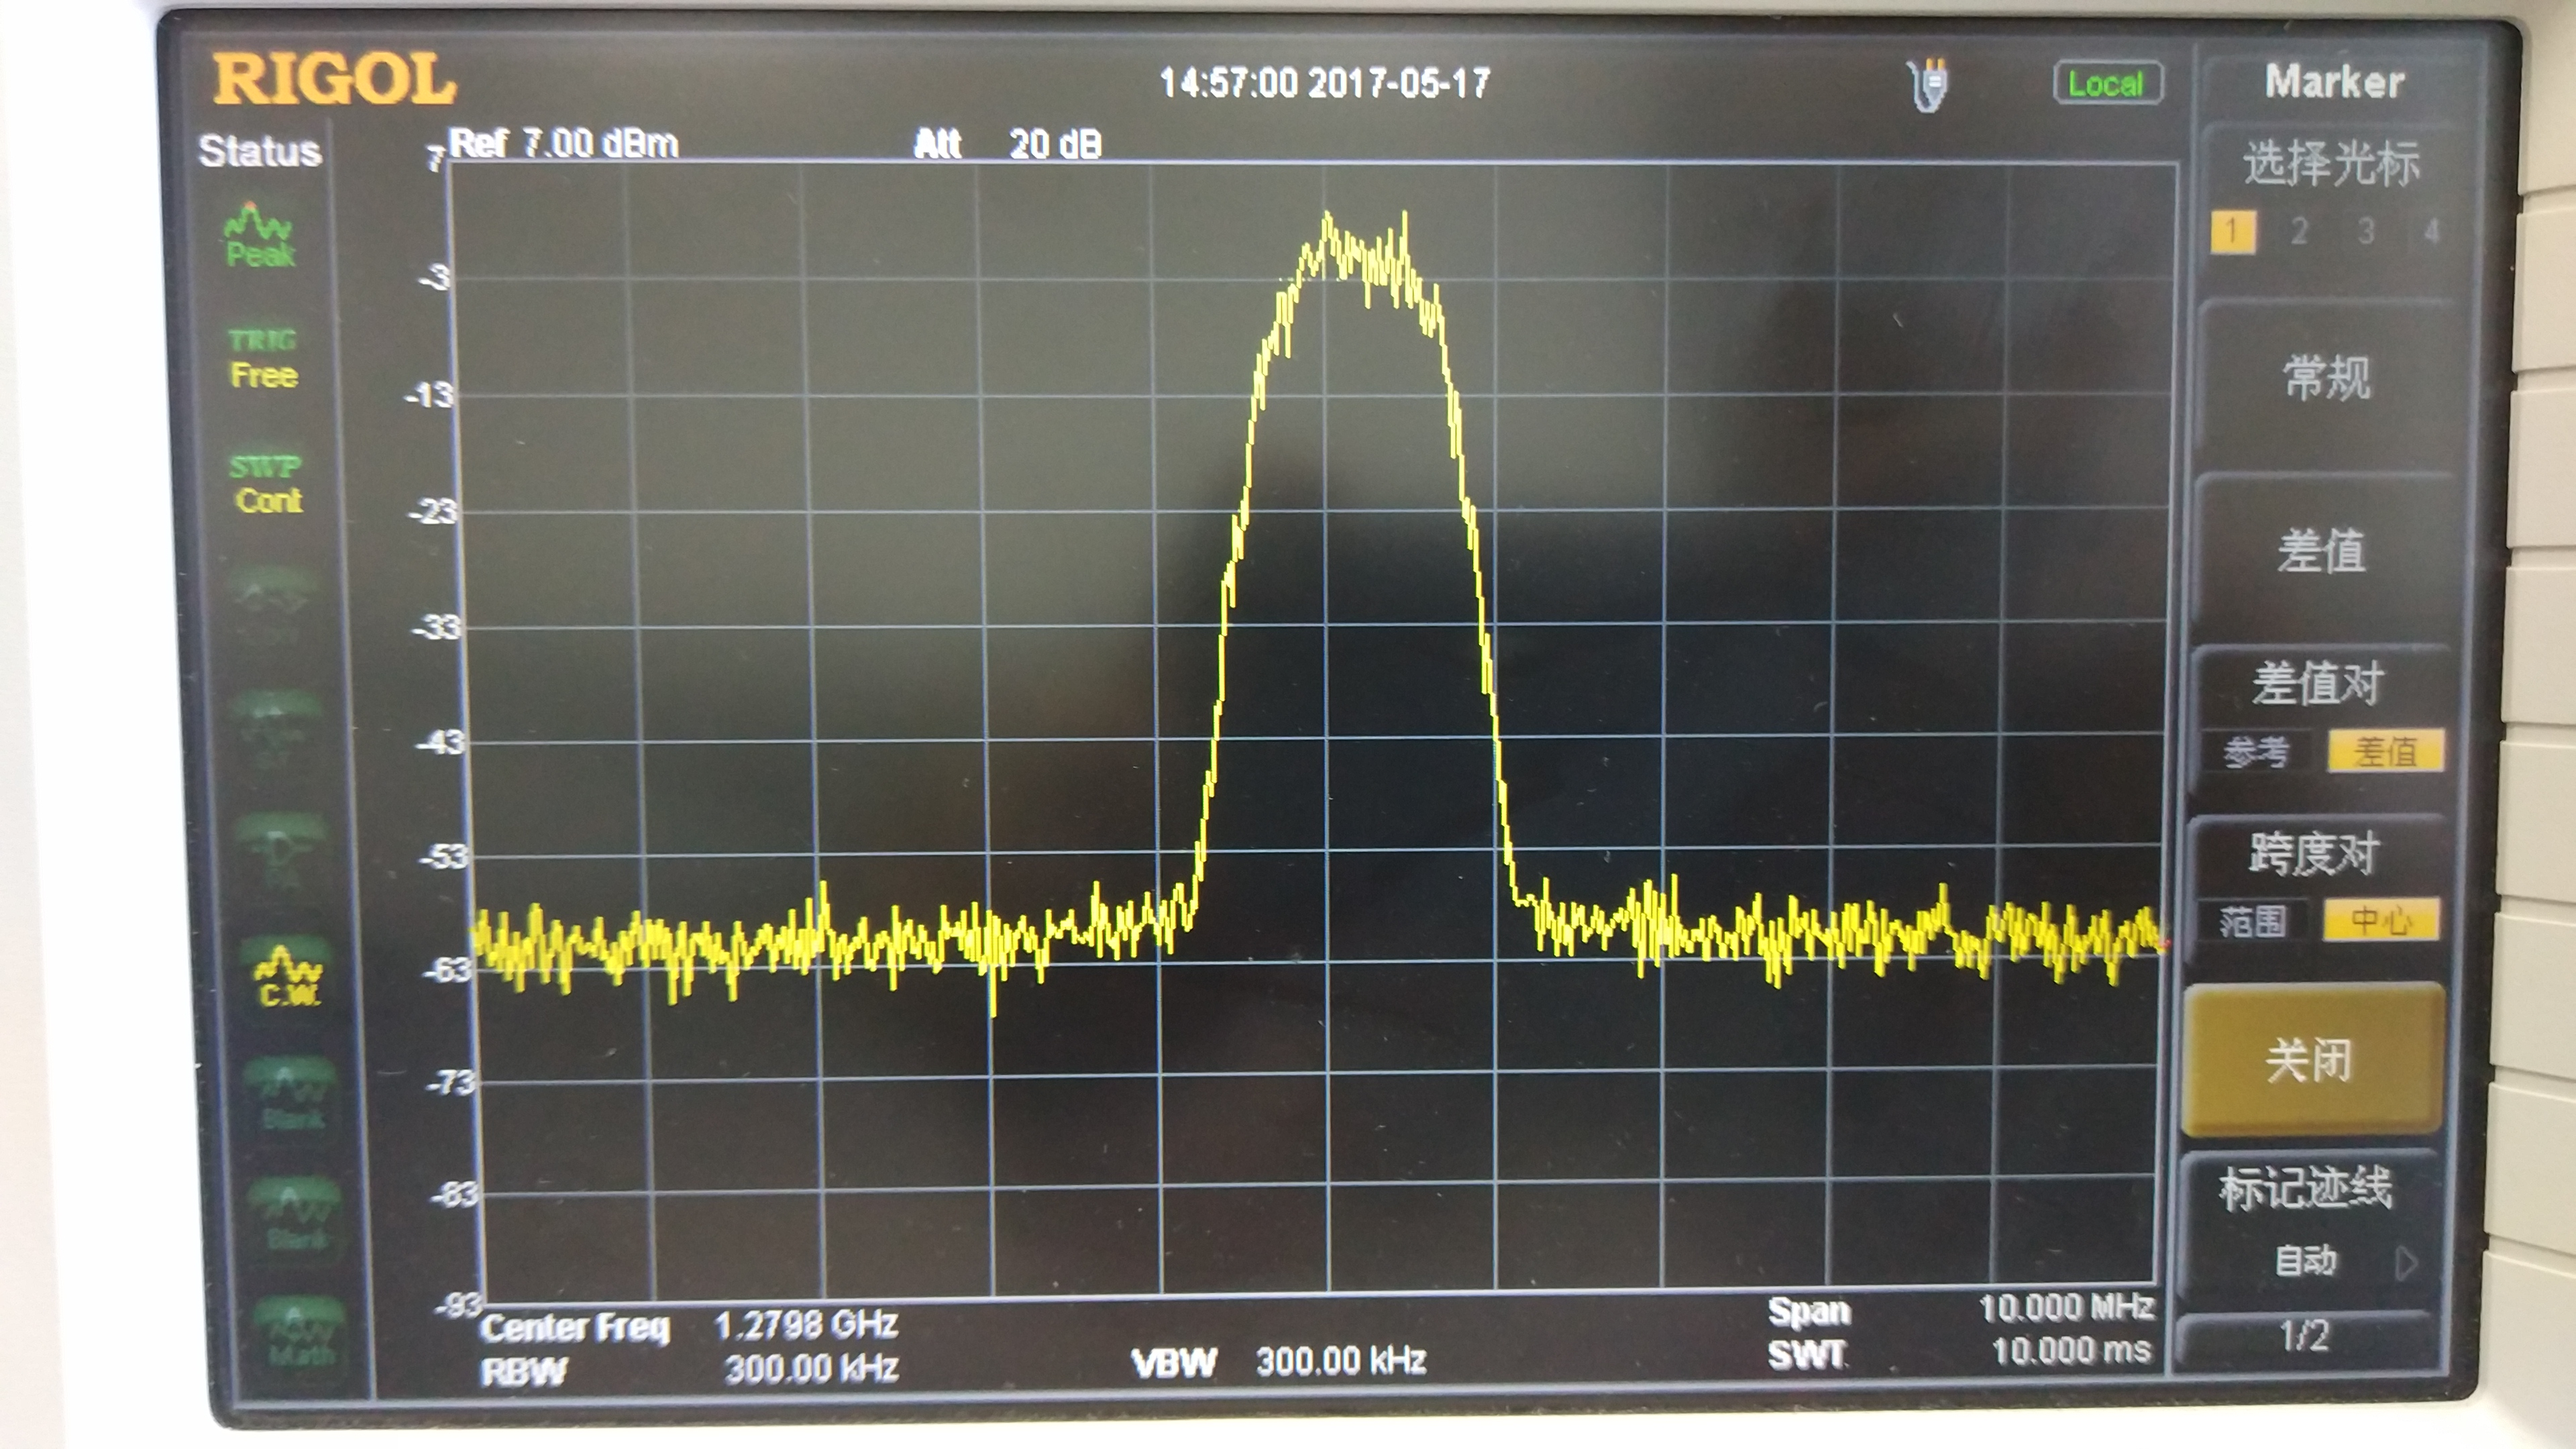
\includegraphics[width=0.4\textwidth]{figures/dvbt_raspi_bandwidth.jpg}
		% 		\label{fig:dvbt_raspi_bandwidth}} \\
		% \end{figure}
